\documentclass[10pt,a4paper]{article}
\usepackage[utf8]{inputenc}

% Define the page margin
\usepackage[margin=3cm]{geometry}

% Better typography (font rendering)
\usepackage{microtype}

% Math environments and macros
\usepackage{amsmath}
\usepackage{amsfonts}
\usepackage{amssymb}
\usepackage{amsthm}

% Define \includegraphics to include graphics
\usepackage{graphicx}

% Draw graphics from a text description
\usepackage{tikz}

% Syntax highlighting
\usepackage{minted}

% Set global minted options
\setminted{linenos, autogobble, frame=lines, framesep=2mm}

% Import the comment environment for orgtbl-mode
\usepackage{comment}

% Do not indent paragraphs
\usepackage{parskip}

\title{Randomized Algorithms, Sheet 10}
\author{Marten Lienen (03670270)}

\begin{document}

\maketitle

\section*{Exercise 10.1}

\begin{proof}
  Fix a bin $i$ and let $X$ be the number of balls in bin $i$.
  For every ball $j$ we can define a variable $Y_{j}$ that is $1$ if ball $j$ lands in bin $i$ and $0$ otherwise.
  This means that $Y_{j}$ are Poisson trials with success probability $\frac{1}{n}$ and $X = \sum_{j} Y_{j}$ and therefore $E[X] = 1$.
  \begin{align*}
    P\left[X \ge \frac{\log n}{\log \log n}\right] & = P\left[X \ge \left(1 + \frac{\log n - \log \log n}{\log \log n}\right)\right]\\
                                                   & = P\left[X \ge \left(1 + \frac{\log \frac{n}{\log n}}{\log \log n}\right)\right]\\
                                                   & \le \frac{\exp\left( \frac{\log \frac{n}{\log n}}{\log \log n} \right)}{\left( \frac{\log n}{\log \log n} \right)^{\frac{\log n}{\log \log n}}}\\
                                                   & = \frac{\exp\left( \frac{\log \frac{n}{\log n}}{\log \log n} \right)}{\frac{(\log n)^{\frac{\log n}{\log \log n}}}{(\log \log n)^{\frac{\log n}{\log \log n}}}}\\
                                                   & = \frac{\exp\left( \frac{\log \frac{n}{\log n}}{\log \log n} \right)}{\frac{\exp\left(\frac{\log n}{\log \log n} \log(\log n)\right)}{\exp\left(\frac{\log n}{\log \log n}\log(\log \log n)\right)}}\\
                                                   & = \frac{\exp\left( \frac{\log \frac{n}{\log n}}{\log \log n} \right) \exp\left(\frac{\log n}{\log \log n}\log(\log \log n)\right)}{n}\\
                                                   & = \frac{\exp\left( \frac{\log\left(\frac{n}{\log n}\right) + \log(n) \log(\log \log n)}{\log \log n} \right)}{n}\\
                                                   & = \frac{\exp\left( \frac{\log(n) + \log(n) \log(\log \log n)}{\log \log n} - 1\right)}{n}\\
                                                   & = \frac{\exp\left( \log(n)\frac{1 + \log(\log(\log(n)))}{\log \log n} - 1\right)}{n}\\
                                                   & < \frac{\exp\left( \log(n)\frac{1 + \log(\log(\log(n)))}{\log \log n} \right)}{n}\\
                                                   & = \frac{1}{n}n^{\frac{1 + \log(\log(\log(n)))}{\log \log n}}\\
  \end{align*}
  This tends towards $0$ just as $\frac{1}{n}$.
  I will leave this here in case this was the desired answer.
\end{proof}

\subsection*{Is it even possible?}

\begin{proof}
  The general form of the Chernoff bound for a sum of Poisson trials is
  \begin{equation*}
    P\left[ X \ge (1 + \delta)\mu \right] \le \min_{t > 0} \frac{e^{(e^{t} - 1)\mu}}{e^{t(1 + \delta)\mu}}
  \end{equation*}
  and we are trying to upperbound this with $\frac{1}{n}$.
  \begin{equation*}
    \min_{t > 0} \frac{e^{(e^{t} - 1)\mu}}{e^{t(1 + \delta)\mu}} < \frac{1}{n}
  \end{equation*}
  Plugging in $\mu = 1$ and $1 + \delta = \frac{\log n}{\log \log n}$ results in
  \begin{equation*}
    \min_{t > 0} \frac{e^{(e^{t} - 1)}}{e^{t \frac{\log n}{\log \log n}}} < \frac{1}{n}
  \end{equation*}
  Combining numerator and denominator and applying the logarithm yields
  \begin{equation*}
    \min_{t > 0} e^{t} - t \frac{\log n}{\log \log n} < \log\left(\frac{1}{n}\right) + 1 = 1 - \log n = \log \frac{e}{n}
  \end{equation*}
  The right hand side is a negative constant for $n > e$ with respect to $t$ and the left hand side is a function $f$ of $t$.
  \begin{equation*}
    f(t) = e^{t} - t \frac{\log n}{\log \log n} \qquad f'(t) = e^{t} - \frac{\log n}{\log \log n} \qquad f''(t) = e^{t}
  \end{equation*}
  $f'$ has a root at $t_{0} = \log\left( \frac{\log n}{\log \log n} \right) > 0$ and $f''$ is positive everywhere, so $f$ has a minimum at $t_{0}$.
  \begin{equation*}
    f(t_{0}) = e^{\log\left( \frac{\log n}{\log \log n} \right)} - \log\left( \frac{\log n}{\log \log n} \right) \frac{\log n}{\log \log n} = \left(1 - \log\left( \frac{\log n}{\log \log n} \right)\right) \frac{\log n}{\log \log n}
  \end{equation*}
  Consequently we can replace the left hand side in the inequality with the actual minimum
  \begin{equation*}
     \left(1 - \log\left( \frac{\log n}{\log \log n} \right)\right) \frac{\log n}{\log \log n} < \log \frac{e}{n}
  \end{equation*}
  Plot \ref{fig:exercise-10-1} shows both sides on the domain $[0, 1000]$ and shows that the minimum is greater than the supposed upper bound after some initial $n_{0} \approx 5$ and continues to fall slower.
  Of course this is not a rigorous proof but for me it is a strong indicator to doubt that $\frac{1}{n}$ is actually an upper bound for the probability of the concerned event.

  \begin{figure}
    \centering
    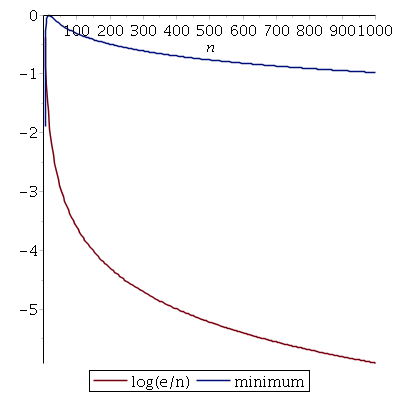
\includegraphics{sheet-10/exercise-10-1}
    \caption{Plot of the minimum and the supposed upper bound}
    \label{fig:exercise-10-1}
  \end{figure}
\end{proof}

\section*{Exercise 10.2}

Let $X_{i}, 1 \le i \le N$ be the vote of each person where $1$ is a vote for impeachment and $0$ against it.
Each $X_{i}$ is a Poisson trial with success probability $p$.
We estimate $p$ as $X = \sum_{i = 1}^{N} \frac{1}{N} X_{i}$ with $E[X] = \mu = p$.
\begin{align*}
  P[|X - p| \le \epsilon p] & = 1 - P[|X - p| > \epsilon p]\\
                            & = 1 - P[X - p > \epsilon p] - P[-X + p > \epsilon p]\\
                            & = 1 - P[X - p > \epsilon p] - P[X - p < -\epsilon p]\\
                            & = 1 - P[X > p + \epsilon p] - P[X < p - \epsilon p]\\
                            & = 1 - P[X > (1 + \epsilon)p] - P[X < (1 - \epsilon)p]\\
                            & = 1 - P[X > (1 + \epsilon)\mu] - P[X < (1 - \epsilon)\mu]
\end{align*}

To apply Chernoff bounds to the terms on the right hand side, we need to compute the Chernoff bounds for a sum of scaled Poisson trials.
A slight modification of the derivation of the moment generating function for sums of Poisson trials leads us to
\begin{equation*}
  M_{X}(t) \le \exp\left( \left(\exp\left(\frac{t}{N}\right) - 1\right)\mu \right) \qquad M_{-X}(t) \le \exp\left( \left(\exp\left(-\frac{t}{N}\right) - 1\right)\mu \right)
\end{equation*}
Furthermore we can adapt the actual bounds to
\begin{equation*}
  P\left( X \ge (1 + \epsilon)\mu \right) \le \left( \frac{e^{\epsilon}}{(1 + \epsilon)^{N(1 + \epsilon)}} \right)^{\mu}
\end{equation*}
and
\begin{equation*}
  P\left( X \le (1 - \epsilon)\mu \right) \le \left( \frac{e^{\epsilon}}{(1 + \epsilon)^{N(1 - \epsilon)}} \right)^{\mu}
\end{equation*}
Applying these to the initial result yields
\begin{align*}
  P[|X - p| \le \epsilon p] & \ge 1 - \left( \frac{e^{\epsilon}}{(1 + \epsilon)^{N(1 + \epsilon)}} \right)^{\mu} - \left( \frac{e^{\epsilon}}{(1 + \epsilon)^{N(1 - \epsilon)}} \right)^{\mu}
\end{align*}

So we get the requested bound when
\begin{equation*}
  \left( \frac{e^{\epsilon}}{(1 + \epsilon)^{N(1 + \epsilon)}} \right)^{\mu} + \left( \frac{e^{\epsilon}}{(1 + \epsilon)^{N(1 - \epsilon)}} \right)^{\mu} < \delta
\end{equation*}
for some $\delta < 1$.
We can increase the exponent in the right denominator to $N(1 + \epsilon)$ to make the left hand side even smaller and be able to put the sum in the numerator.
\begin{equation*}
  \frac{2e^{\epsilon\mu}}{(1 + \epsilon)^{N(1 + \epsilon)\mu}} < \delta
\end{equation*}
Solving for $N$ yields
\begin{equation*}
  \frac{2e^{\epsilon\mu}}{\delta} < (1 + \epsilon)^{N(1 + \epsilon)\mu} \Leftrightarrow N > \log_{(1 + \epsilon)^{(1 + \epsilon)\mu}}\left( \frac{2e^{\epsilon\mu}}{\delta} \right) = \log_{(1 + \epsilon)^{(1 + \epsilon)p}}\left( \frac{2e^{\epsilon p}}{\delta} \right)
\end{equation*}

Plot \ref{fig:exercise-10-2-plot} of the lower bound shows that you need to survey at least 68 independent people to get an estimate that is within a relative error bound of 10\% around the real $p$ with a probability of 95\% when you assume that the real $p$ is between $0.2$ and $0.8$.

\begin{figure}
  \centering
  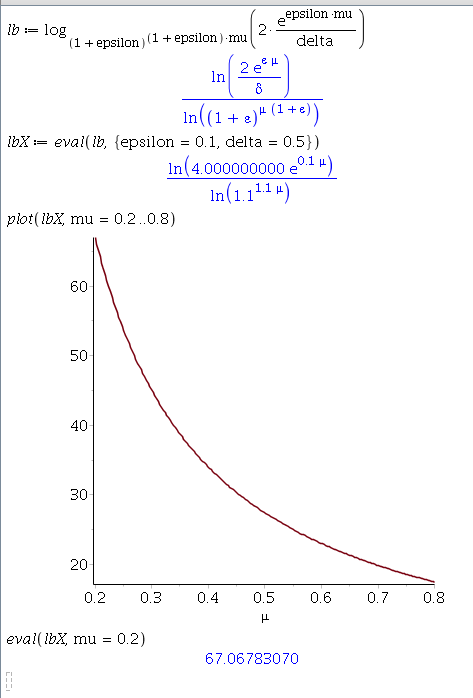
\includegraphics[width=\textwidth]{sheet-10/exercise-10-2}
  \caption{Plotted with maple}
  \label{fig:exercise-10-2-plot}
\end{figure}

\section*{Exercise 10.3}

\begin{proof}
  The question if the generated permutations are uniformly random can be rephrased as: If you draw $n$ unique values from the black box, is the probability that you draw the $j$th largest number of the $n$ in the $i$th draw $\frac{1}{n}$?
  The answer is \emph{yes} because
\end{proof}

Let $X_{i}, 1 \le i \le n$ be the number of calls to the black box that are necessary to determine the $i$th value of $f$.
The $X_{i}$ can be modelled as geometric distributions with success probability $p_{i} = \frac{k - (i - 1)}{k} = \frac{k - i + 1}{k}$ because there are $k - (i - 1)$ numbers that have not been drawn for the previous $i - 1$ positions.
\begin{equation*}
  P[X_{i} = j] = \left( \frac{i - 1}{k} \right)^{j - 1}\frac{k - i + 1}{k} \qquad E[X_{i}] = \frac{k}{k - i + 1}
\end{equation*}
Let $X = \sum_{i} X_{i}$.
\begin{equation*}
  E[X] = \sum_{i} E[X_{i}] = \sum_{i = 1}^{n} \frac{k}{k - i + 1} = k \sum_{i = 1}^{n} \frac{1}{k - i + 1} = k \cdot \left( H_{k} - H_{k - n} \right)
\end{equation*}
For $k = n$ we get $E[X] = n H_{n}$ and for $k = 2n$ we get $E[X] = 2n \cdot (H_{2n} - H_{n})$.

Let $k = 2n$.
The probability that a call to the black box yields a unique result, i.e. the success probability of an $X_{i}$ is $\frac{2n - i + 1}{2n}$ for $1 \le i \le n$.
This is lower bounded by $\frac{2n - n + 1}{2n} = \frac{n + 1}{2n} > \frac{n}{2n} = \frac{1}{2}$.
Therefore for each call to the black box a value is assigned with probability at least $\frac{1}{2}$.

\begin{align*}
  E[e^{tX_{i}}] & = \sum_{j = 1}^{\infty} e^{tj} \cdot P[X_{i} = j]\\
                & = \sum_{j = 1}^{\infty} e^{tj} \cdot \left( 1 - p_{i} \right)^{j - 1}p_{i}\\
                & = \sum_{j = 1}^{\infty} e^{tj} \cdot (1 - p_{i})^{j} (1 - p_{i})^{-1} p_{i}\\
                & = \frac{p_{i}}{1 - p_{i}} \sum_{j = 1}^{\infty} \left( e^{t}(1 - p_{i}) \right)^{j}\\
                & = \frac{p_{i}}{1 - p_{i}} \left( \frac{1}{1 - e^{t}(1 - p_{i})}  - 1\right) \qquad \textit{for $t < -\log(1 - p_{i})$}\\
                & = \frac{p_{i}}{1 - p_{i}} \frac{e^{t}(1 - p_{i})}{1 - e^{t}(1 - p_{i})}\\
                & = \frac{e^{t}p_{i}}{1 - e^{t}(1 - p_{i})}
\end{align*}

The derivative with respect to $p_{i}$ is
\begin{align*}
  \left( E[e^{tX_{i}}] \right)' = \frac{e^{t}(1 - e^{t})}{\left( 1 - e^{t}(1 - p_{i}) \right)^{2}}
\end{align*}
which is strictly negative for all $t > 0$ because $e^{t} > 1 \Leftrightarrow t > 0$.
Therefore $E[e^{tX_{i}}]$ is upper bounded by the smallest possible value for $p_{i}$ which is $\frac{1}{2}$ is this case.
\begin{equation*}
  E[e^{tX_{i}}] \le \frac{e^{t}\frac{1}{2}}{1 - e^{t}(1 - \frac{1}{2})} = \frac{e^{t}\frac{1}{2}}{1 - \frac{e^{t}}{2}} = \frac{e^{t}}{2 - e^{t}}
\end{equation*}

\begin{align*}
  E[e^{tX}] & = \prod_{i = 1}^{n} E[e^{tX_{i}}]\\
            & \le \prod_{i = 1}^{n} \frac{e^{t}}{2 - e^{t}}\\
            & = \left(\frac{e^{t}}{2 - e^{t}}\right)^{n}
\end{align*}

\begin{align*}
  P[X \ge 4n] & = P[e^{tX} \ge e^{4tn}]\\
              & \le \frac{E[e^{tX}]}{e^{4tn}}\\
              & \le \frac{\left(\frac{e^{t}}{2 - e^{t}}\right)^{n}}{e^{4tn}}\\
              & = \frac{1}{(2 - e^{t})^{n}e^{3tn}}\\
              & = \left(\frac{1}{(2 - e^{t})e^{3t}}\right)^{n}
\end{align*}
This is true for all $0 < t < -\log(1 - p_{i}) \le -\log\left( 1 - \frac{1}{2} \right) = \log(2)$.
The derivative of the denominator is
\begin{equation*}
  \left( (2 - e^{t})e^{3t} \right)' = e^{3t}(6 - 4e^{t})
\end{equation*}
which has one root at $t_{0} = \log(\frac{3}{2})$.
The denominator itself evaluates to $1$ and $0$ at the boundaries $0$ and $\log(2)$ but to $\frac{1}{2}\left( \frac{3}{2} \right)^{3} = \frac{3^{3}}{2^{4}} = 1.6875$ at $t_{0}$.
Therefore it has a local maximum at $t_{0}$.
Plugging $t_{0}$ into the high probability bound yields
\begin{align*}
  P[X \ge 4n] \le \left( \frac{2^{4}}{3^{3}} \right)^{n}
\end{align*}

\section*{Exercise 10.4}

\begin{proof}
  \begin{equation*}
    E[X] = \sum_{i = 1}^{n} E[X_{i}] = \sum_{i = 1}^{n} (1 - p_{i})p_{i} - p_{i}(1 - p_{i}) = \sum_{i = 1}^{n} 0 = 0
  \end{equation*}
  \begin{align*}
    E[e^{tX}] & = \prod_{i = 1}^{n} E[e^{tX_{i}}]\\
              & = \prod_{i = 1}^{n} \left(p_{i}e^{t(1 - p_{i})} + (1 - p_{i})e^{-tp_{i}}\right)\\
    \intertext{Use the inequality from the hint}
              & \le \prod_{i = 1}^{n} e^{\frac{t^{2}}{8}} = e^{\frac{n}{8}t^{2}}\\
  \end{align*}
  The same way you see that $E[e^{-tX}] \le e^{\frac{n}{8}t^{2}}$ because you can substitute $t' = -t$ and during resubstitution the minus vanishes since $t'$ only appears quadratically.
  \begin{align*}
    P[|X| \ge a] & = P[X \ge a] + P[-X \ge a]\\
                 & = P[e^{tX} \ge e^{ta}] + P[e^{-tX} \ge e^{ta}]\\
                 & \le \frac{E[e^{tX}]}{e^{ta}} + \frac{E[e^{-tX}]}{e^{ta}}\\
                 & \le \frac{e^{\frac{n}{8}t^{2}}}{e^{ta}} + \frac{e^{\frac{n}{8}t^{2}}}{e^{ta}}\\
                 & = 2 \frac{e^{\frac{n}{8}t^{2}}}{e^{ta}} = 2e^{\frac{n}{8}t^{2} - at}
  \end{align*}
  for any $t > 0$.
  Considering the desired form of the upper bound we have to solve
  \begin{equation*}
    \frac{n}{8}t^{2} - at = -2 \frac{a^{2}}{n} \Leftrightarrow t^{2} - \frac{8a}{n}t + \frac{16a^{2}}{n^{2}} = 0 \Leftrightarrow t = \frac{4a}{n} \pm \sqrt{\left( \frac{4a}{n} \right)^{2} - \frac{16a^{2}}{n^{2}}} \Leftrightarrow t = \frac{4a}{n}
  \end{equation*}
  Plugging in $t = \frac{4a}{n}$ yields
  \begin{align*}
    P[|X| \ge a] & \le 2e^{\frac{n}{8}\left( \frac{4a}{n} \right)^{2} - a \frac{4a}{n}} = 2e^{\frac{n}{8} \frac{16a^{2}}{n^{2}} - \frac{4a^{2}}{n}} = 2e^{\frac{2a^{2}}{n} - \frac{4a^{2}}{n}} = 2e^{-2\frac{a^{2}}{n}}
  \end{align*}
\end{proof}

\end{document}
